% Pontos A(0,0), B(2,0), C(3,0)
% 5kN aplicada para baixo em B
% Engastado em A

\documentclass[tikz]{standalone}
\usepackage{stanli}
\usetikzlibrary{calc}

\begin{document}
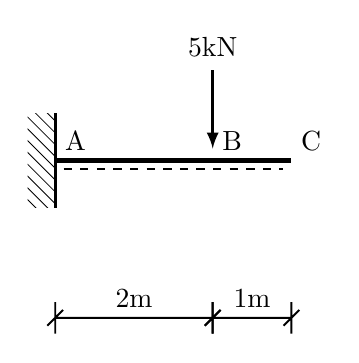
\begin{tikzpicture}
    % Definição dos pontos
    \point{A}{0}{0}
    \point{B}{2}{0}
    \point{C}{3}{0}

    % Definição dos apoios
    % Engastado em A (parede à esquerda: rotação = -90)
    \support{3}{A}[-90]

    % Definição da viga
    \beam{1}{A}{C}

    % Carga pontual
    % 5kN para baixo (90) em B
    \load{1}{B}[90]

    % Notações e Etiquetas
    \notation{1}{A}{A}[above right]
    \notation{1}{B}{B}[above right]
    \notation{1}{C}{C}[above right]
    
    % Regra: carga para baixo utiliza [above=12mm]
    \notation{1}{B}{5kN}[above=12mm]

    % Dimensionamento
    \dimensioning{1}{A}{B}{-20mm}[2m]
    \dimensioning{1}{B}{C}{-20mm}[1m]
\end{tikzpicture}
\end{document}